% najpierw jest wstep, załączenie potrzebnych pakietów itp.
\documentclass[a4paper, 10pt]{article}

%polskie znaki
\usepackage[polish]{babel}
\usepackage[utf8]{inputenc}
\usepackage[OT4]{fontenc}

%wieksze mozliwosci zmiany wygladu strony, pakiet do wstawiania linków
\usepackage{geometry}
\usepackage{ulem}

\RequirePackage{url}
\usepackage{subfig}
\usepackage{placeins}
% ladne wciecia akapitow i odstepy, mozna wykasowac wedle uznania;)
\setlength{\parindent}{0cm}
\setlength{\parskip}{3mm plus1mm minus1mm}

%mniejsze marginesy
\geometry{verbose,a4paper,tmargin=2.4cm,bmargin=2.4cm,lmargin=2.4cm,rmargin=2.4cm}
\usepackage{graphicx} % wstawianie obrazkow

\newcommand{\ang}[1]{(ang. #1\/)}
%%%%%%%%%%%%%%%%%%%%%%%%%%%%%%%%%%%%%%%%%%%%%%%%

\title{{\bf {Inteligentne systemy informacyjne }} \\ {\large Dokumentacja projektu}}
\date{\today}
\author{Filip Nabrdalik}


%%%%%%%%%%%%%%%%%%%%%%%%%%%%%%%%%%%%%%%%%%%%%%%%
\begin{document}
\bibliographystyle{abbrv}
%%%%%%%
\null  % Empty line
\nointerlineskip  % No skip for prev line
\vfill
\let\snewpage \newpage
\let\newpage \relax
\maketitle %wstawienie tytulu, daty i autora
\let \newpage \snewpage
\vfill
\break % page break
%%%%%%%%%%%%%%%%%%%%%%%%%%%%%



\tableofcontents

\newpage






\section{Treść zadania}

{\bf{Zadanie 7}}

{\it Zaprojektować i zaimplementować środowisko do Conwey’a „Game of Life”}


\section{Game of Life}

Game of Life \cite{gol} w skrócie Life, jest automatem komórkowym zaprojektowanym w roku 1970 przez brytyjskiego matematyka Johna Conwaya.
Gra odbywa się praktycznie bez udziału gracza. Gracz ustala początkową konfiguracje komórek, a następnie obserwuje ewolucję
populacji w kolejnych krokach.

 {\bf{Zasady gry Life }}

Istnieje kilka wzorców generowania, jednak oryginalna wersja
gry opiera się na kilku prostych regułach:

\begin{itemize}
  \item żywa komórka umiera, jeśli w swoim sąsiedztwie ma mniej niż 2 żywych sąsiadów (niedostateczne zaludnienie),
  \item żywa komórka przetrwa do następnej generacji, jeśli w swoim sąsiedztwie ma 2 lub 3 żywych sąsiadów,
  \item żywa komórka umiera do następnej generacji, jeśli w swoim sąsiedztwie ma więcej niż 3 żywych sąsiadów (przeludnienie),
  \item martwa komórka ożywa, jeśli ma w swoim sąsiedztwie 3 żywe komórki (rozmnażanie).
\end{itemize}

Wynikają one ze wstępnych założeń Johna Conwaya, czyli: braku nagłego wzrostu populacji, istnienia małych struktur populacji (które ewoluują chaotycznie),
oparciu o uniwersalny konstruktor von Neumanna \cite{vnc} oraz maksymalnego uproszczenia reguł gry.

{\bf{Struktury}}
 
Pierwsze proste struktury stałe \ang{still lifes} oraz oscylatory \ang{oscillators} występujące w Life zostały odkryte bez użycia komputerów w 1970 roku. 
Conway odkrył też, że struktura R-pentomino potrzebuje, aż 1103 generacji do ustabilizowania podczas, których wystrzeliwuje 6 szybowców, 
a w fazie stabilnej ma populacje 116 komórek. 

Obecnie przy wykorzystaniu mocy obliczeniowej komputerów są odkrywane coraz to nowe struktury. Ich podział wygląda następująco:

\begin{itemize}
  \item struktury stałe - nie ulegają zmianom podczas kolejnych generacji
  \item oscylatory - struktury która wracają do pierwotnej konfiguracji po określonej liczbie generacji,
  \item statki kosmiczne \ang{spaceships}- struktury która pojawiają się w pierwotnej konfiguracji z przemieszeniem po określonej liczbie generacji,
  \item matuzalemy \ang{methuselahs}- struktury, które znacznie rozrastają się i stabilizują po dużej ilości generacji,
  \item stacje kosmiczne \ang{guns}- przechwytujące lub wystrzeliwujące statki kosmiczne,
  \item parowozy \ang{puffers}- statki kosmiczne pozostawiające po sobie złom,
  
\end{itemize}

 



\newpage

\section{Wybrane struktury}


W Game of Life można wyróżnić wielu charakterystycznych struktur, .


{\bf{Struktury stałe}}


 \begin{figure}[ht]
  
  
	\centering
	\subfloat[Struktury stałe]{%
	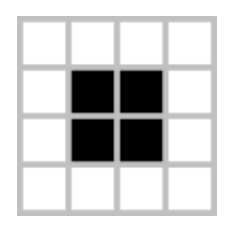
\includegraphics[width=15mm]{rys/block.eps}
	
	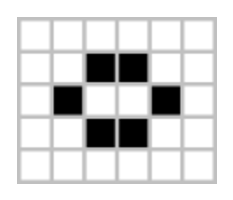
\includegraphics[width=15mm]{rys/beehive.eps}}
	\quad
 	
	
 \end{figure}
 
 {\bf{Oscylatory}}

 \begin{figure}[!ht]
  
  
	\centering
	\subfloat[Blinker 2 fazy]{%
	\includegraphics[width=15mm]{rys/blinker1.eps}
	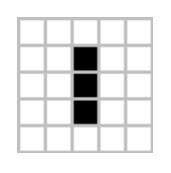
\includegraphics[width=15mm]{rys/bliker2.eps}}

	\quad
 	
	
 \end{figure}
 

 
 \begin{figure}[!ht]
  
  
	\centering
	\subfloat[Beacon 2 fazy]{%
	\includegraphics[width=15mm]{rys/beacon1.eps}
	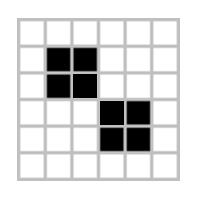
\includegraphics[width=15mm]{rys/beacon2.eps}}

	\quad
 	
	
 \end{figure}


  
 \begin{figure}[!ht]
  
  
	\centering
	\subfloat[Żaba 2 fazy]{%
	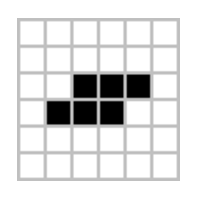
\includegraphics[width=15mm]{rys/toad1.eps}
	\includegraphics[width=15mm]{rys/toad2.eps}}

	\quad
 	
	
 \end{figure}
 
  \FloatBarrier
  
{\bf{Statki kosmiczne}}




  
 \begin{figure}[!ht]
  
  
	\centering
	\subfloat[Szybowiec \ang{glider} 4 oscylacje i ruch]{%
	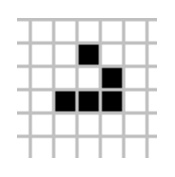
\includegraphics[width=15mm]{rys/glider1.eps}
	\includegraphics[width=15mm]{rys/glider2.eps}}

	\quad
 	
	
 \end{figure}

 \begin{figure}[!ht]
  
  
	\centering
	\subfloat[Szybowiec \ang{glider} 3 oscylacje i ruch]{%
	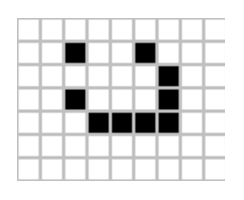
\includegraphics[width=15mm]{rys/lwss1.eps}
	\includegraphics[width=15mm]{rys/lwss2.eps}}

	\quad
 	
	
 \end{figure}


\section{Środowisko Game of Life}

Program do gry Life został zrealizowany pod systemem Linux w języku C z wykorzystanie biblioteki ncurses  \cite{nc}.
Aplikacje należy uruchomić poleceniem: {\it{life Y X }}\quad, gdzie X oraz Y to odpowiednio szerokość i wysokość świata gry (maksymalnie wysokość i szerokość terminala).
Pole gry zostało zrealizowane w postaci siatki kolumn i linii.

Użytkownik może poruszać się po polu gry klawiszami strzałek i w dowolnej rundzie uśmiercić bądź ożywić
komórkę za pomocą klawisza spacji. Przechodzenie do kolejnych generacji odbywa się po wciśnięciu klawisza n.
Wyjście z gry następuje po użyciu klawisza q.

Użytkownik może wygenerować losowe ustawienie żywych komórek za pomocą klawisza r. 

Dodatkowo niektórym strukturom zostały przypisane klawisze, w celu łatwego wstawienia ich do świata gry:

 \begin{itemize}
  \item klawisz a - szybowiec,
  \item klawisz s - LWSS, czyli lekki statek kosmiczny,
  \item klawisz z - żaba,
  \item klawisz x - blinker,
   \item klawisz w - blok,
  \item klawisz e - lotniskowiec.
\end{itemize}



\section{Wnioski}




Podczas symulacji zwróciłem uwagę na charakterystykę populacji w grze. Duże i geste populacje nie maja szans na przeżycie, 
jednak małe, czy mnie gęste oscylatory i struktury stałe zapewniają ciągłość populacji w następnych generacjach i są symetryczne. 

Ciekawym okazał się eksperyment ze zderzeniami populacji, często tak powstałe struktury szybko obumierały wysyłając 
szybowce ewakuacyjne na plansze gry, które łączyły się z pozostałymi populacjami. 

Do dziś odkrywane są coraz to nowe struktury różniące się od siebie charakterystyką i częstością występowania. 
Gra Life jest dobrym przykładem emergencji i samo-organizacji. Zwraca tym samym na siebie uwagę
badaczy z wielu dziedzin nauki takich, jak ekonomia, biologia, biochemia, matematyka i statystyka.











%BIBLIOGRAFIA
\nocite{*}
\bibliography{bibliografia}


\end{document}


